\chapter{Metodologia}
\label{chapter:metodologia}

\section{Definição dos parâmetros de entrada e saída}

\subsection{Parâmetros de entrada}\label{subsec:par}

A princípio, a definição dos parâmetros adotados para gerar a base de dados de simulações para o desenvolvimento do metamodelo foram obtidos a partir do banco de dados com 153 edificações de escritórios com \acrfull{vn} disponibilizado por \citeonline{Neves2019}.  		
Dentre as informações  disponíveis no banco de dados, obtém-se:

\begin{itemize}
	\item orientação solar do edifício;
	\item número de pavimentos;
	\item forma dos pavimentos e das salas;
	\item áreas das salas;  % dos pavimentos e
	\item altura do pé-direito das salas;
	\item relações entre as dimensões dos pavimentos e entre as dimensões das salas;
	\item absortância das paredes externas; % 0.2 - 0.8
	%			\item espessura das paredes externas;
	\item cor da cobertura;
	\item tipo de vidro nas janelas;
	\item tipo de esquadria;
	\item fator de abertura das janelas;
	%			\item altura das esquadrias;
	\item \acrfull{paf};  % 0 - 80
	\item tipo de sombreamento;  % 0 - 80
	\item tipo de estratégia de \acrlong{vn} (unilateral ou cruzada).
\end{itemize} 

Os valores desses parâmetros foram observados através de suas distribuições de ocorrência. Desta forma definiu-se os limites mínimos e máximos para o desenvolvimento das simulações termoenergéticas, com parâmetros variando de acordo com o que se encontra comumente em edifícios reais. Como as edificações do banco de dados localizam-se na cidade de São Paulo, esse foi o clima para qual o metamodelo foi desenvolvido.

Certas informações não estão disponibilizadas pelo banco de dados analisado, como algumas relacionadas às propriedades termofísicas dos materiais da envoltória, às densidades de potência de iluminação e equipamentos, e aos padrões e taxas de ocupação. Frente a essa limitação, os valores desses parâmetros foram definidos a partir da \acrlong{inic} \cite{INIC}. %, através da Tabela 4.1, da Tabela A.1 do anexo A e da Tabela B.I.1 do anexo B.  % Hora início e fim: 8 - 18,  INI-C

A Tabela \ref{table:paramconst} apresenta os parâmetros que mantiveram-se com valores constantes no desenvolvimento do trabalho. Esses valores foram escolhidos a partir do que é apresentado na \citeonline{INIC} para a simulação das edificações nas condições de referência. A cobertura tem suas propriedades termofísicas baseadas na consideração de uma laje de concreto de 10 cm de espessura e telha de fibrocimento, separadas por uma câmara de ar. O padrão de ocupação foi definido de acordo com o que é estabelecido para a análise de conforto térmico em edificações de escritórios pelo método simplificado, considerando-se apenas dias de semana. Valores relacionados às propriedades termofísicas do piso em contato com solo e da laje entre pavimentos não são especificados pela \acrshort{inic} para o caso de referência, portanto foi considerado, para ambos os casos, uma laje de concreto de 12cm de espessura com uma camada de piso cerâmico.

\begin{table}[h]
	\centering
	\caption{Parâmetros com valores constantes}
	\label{table:paramconst}
	\begin{tabular}{|l |c |c |}
		\hline
		\textbf{Parâmetros} & \textbf{Valores} & \textbf{Unidades} \\
		\hline
		Capacidade térmica da cobertura & 233 & kJ/m$^2$K \\
		\hline
		Transmitância da cobertura & 2,06 & W/m$^2$K \\
		\hline
		Capacidade térmica do piso / laje & 306 & kJ/m$^2$K \\
		\hline
		Transmitância do piso / laje & 4,30 & W/m$^2$K \\
		\hline
		Transmitância do vidro & 5,7 & W/m$^2$K \\
		\hline 
		Densidade de potência de iluminação & 14 & W/m$^2$ \\
		\hline 
		Densidade de potência de equipamentos & 97 & W/pessoa \\
		\hline 
		Hora de início de ocupação & 8 & horas \\
		\hline 
		Hora final de ocupação & 18 & horas \\
		\hline 
	\end{tabular}
	%			\begin{flushleft}
	%				Fonte: \citeauthoronline{INIC} \cite{INIC}, adaptado pelo autor.
	%			\end{flushleft}				
\end{table}

Os parâmetros da Tabela \ref{table:paraminic} tiveram seus limites mínimos e máximos baseados nos limites apresentados na \citeonline{INIC} para a aplicação do método simplificado. Tanto edificações condicionadas artificialmente, quanto edificações naturalmente ventiladas ou híbridas têm limites semelhantes para a aplicação do método.
A única excessão é a taxa de ocupação, que é sempre considerada com o valor fixo de 0,10 pessoas/m$^2$ na \citeonline{INIC}. No entanto, sabendo-se da influência que a carga térmica proveniente dos ocupantes e equipamentos elétricos pode ter nas temperaturas internas das zonas térmicas, optou-se por variar a taxa de ocupação entre a metade e o dobro do que é definido pela Instrução Normativa. A densidade de potência dos equipamentos foi definida com um valor constante, mas varia de acordo com a taxa de ocupação, como apresentado previamente na Tabela \ref{table:paramconst}.

\begin{table}[h]
	\centering
	\caption{Limites mínimos e máximos de valores dos parâmetros variáveis não disponíveis no banco de dados}
	\label{table:paraminic}
	\begin{tabular}{|l |c |c |}
		\hline
		\textbf{Parâmetros} & \textbf{Faixa de valores} & \textbf{Unidades} \\
		\hline
		Capacidade térmica da parede & 0,22 - 450 & kJ/m$^2$K \\
		\hline
		Transmitância da parede & 0,50 - 4,40 & W/m$^2$K \\
		\hline
		Fator solar do vidro & 0,20 - 0,87 & - \\
		\hline 
		Ângulo horizontal de sombreamento & 0 - 80 & graus \\
		\hline 
		Taxa de ocupação & 0,05 - 0,20 & pessoas/m$^2$ \\
		\hline 
	\end{tabular}
	%			\begin{flushleft}
	%				Fonte: \citeauthoronline{INIC} \cite{INIC}, adaptado pelo autor.
	%			\end{flushleft}				
\end{table}

\subsection{Parâmetro de saída}

A variável de saída do metamodelo desenvolvido é a \acrfull{ehf}. Neste trabalho, o indicador escolhido para o limite superior da temperatura é estabelecido pelo método de conforto adaptativo da \citeonline{ASHRAEStandard552017}, para 80\% de aceitabilidade entre os ocupantes. O desconforto por frio não foi considerado.
A Figura \ref{fig:temp_means} apresenta as temperaturas externas da cidade de São Paulo, com suas médias mensais, e os limites superiores de temperatura pelo método de conforto adaptativo da \citeonline{ASHRAEStandard552017}, para 80\% de aceitabilidade entre os ocupantes.
O arquivo climático utilizado para o desenvolvimento do gráfico é o TMYx 2003-2017. 
Observando-se os valores das temperaturas externas entre às 8 horas e 18 horas ao longo do ano, obtém-se um \acrshort{ehf} igual a 0,124.

\begin{figure}[H]
	%	\vspace{0pt}
	\centering
	\caption{Temperaturas externas da cidade de São Paulo, e limites superiores de aceitabilidade}
	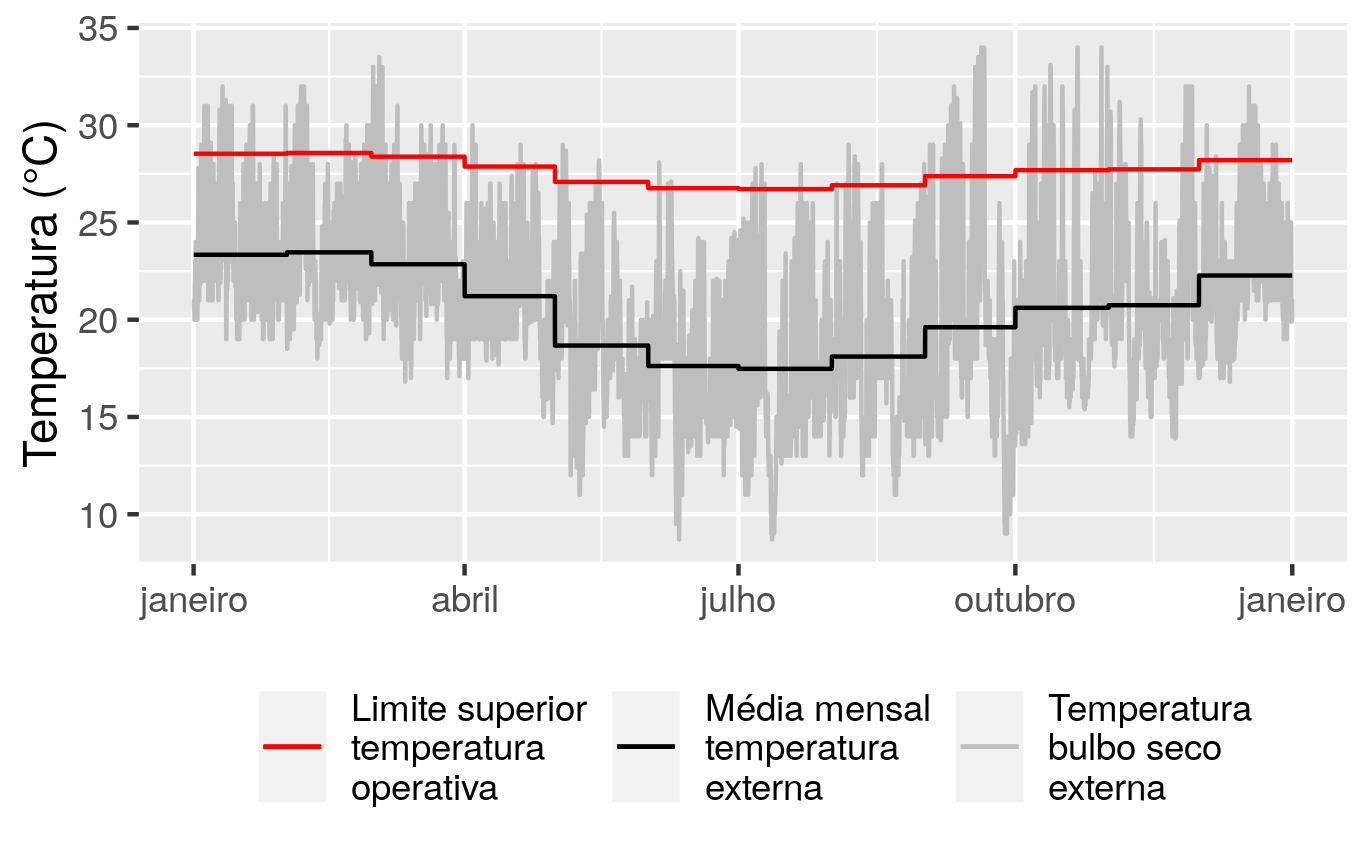
\includegraphics[width=.8\linewidth]{img/temp_means.png}
	\label{fig:temp_means}
	%	\vspace{-5pt}
\end{figure}

A partir dos resultados das simulações, para cada \textit{timestep} com ocupação na sala, foi calculado se as temperaturas operativas das zonas térmicas ultrapassaram o limite superior determinado pelo método adaptativo da \citeonline{ASHRAEStandard552017}. A fração de horas de desconforto foi obtida para cada zona térmica modelada, de acordo com a Equação \ref{eq:EHF}:

\begin{equation}
\label{eq:EHF}
EHF = \frac{timesteps_{sup}}{timesteps_{ocup}}
\end{equation}

Onde:

$EHF$ é igual a fração de horas de desconforto por calor na zona térmica;

\gls{tssup} é igual ao número de \textit{timesteps} em que há ocupação na zona térmica e a temperatura operativa ultrapassa o limite superior determinado pelo método adaptativo;

\gls{tsocup} é igual ao número de \textit{timesteps} em que há ocupação na zona térmica.
\\

Para avaliar o potencial do uso de ventiladores, o movimento do ar foi considerado no desenvolvimento do metamodelo.
A \citeonline{ASHRAEStandard552017} considera um aumento no limite superior da faixa de conforto térmico de acordo com a velocidade do ar.
O aumento de aceitabilidade da temperatura operativa foi considerado para os três valores de velocidade do ar apresentados na Tabela \ref{table:var}, além da possibilidade se assumir o valor de velocidade do ar igual a zero, caso o uso de ventilador não tenha sido considerado.

\begin{table}[h]
	\centering
	\caption{Aumento no limite superior da faixa de conforto em relação à velocidade do ar}
	\label{table:var}
	\begin{tabular}{|c |c |}
		\hline
		\textbf{Velocidade média do ar} & \textbf{Temperatura} \\
		\hline
		0,6 m/s & 1,2 $^{\circ}C$ \\
		\hline
		0,9 m/s & 1,8 $^{\circ}C$ \\
		\hline
		1,2 m/s & 2,2 $^{\circ}C$ \\
		\hline 
	\end{tabular}
	\source{\citeonline{ASHRAEStandard552017}}
\end{table}

Como o modelo de \acrlong{vn} do programa EnergyPlus não calcula a velocidade do ar dentro das zonas, a consideração foi aplicada após as simulações, no momento da avaliação do conforto térmico em cada \textit{timestep}. A consideração da velocidade do ar foi realizada de acordo com a Equação \ref{eq:Tsup}.

\begin{equation}
\label{eq:Tsup}
T_{sup,v} = T_{sup} + T_{v_{ar}}
\end{equation}

Onde:

\gls{tsupv} é igual à temperatura limite superior na faixa de conforto, considerando-se a velocidade do ar ($^{\circ}C$);

\gls{tsup} é igual à temperatura limite superior na faixa de conforto definida pelo método adaptativo, sem considerar a velocidade do ar ($^{\circ}C$);

\gls{tvar} é igual à margem extra de temperatura permitida pela consideração da velocidade do ar ($^{\circ}C$).
\\

\section{Simulação termoenergética}

\subsection{Simulação detalhada}

Sabendo-se que o metamodelo estima o conforto térmico baseado no método adaptativo da \citeonline{ASHRAEStandard552017}, o principal dado de saída a se obter nas simulações foi a temperatura operativa da zona térmica, assim como a temperatura do ar externo. Portanto, todo o desenvolvimento das simulações termoenergéticas do trabalho foi voltado para que se obtivesse, com boa exatidão, a temperatura operativa das zonas térmicas e, posteriormente, a sua relação com a temperatura do ar externo, chegando-se ao indicador de conforto térmico.

%		A Tabela \ref{table:parametros} apresenta os parâmetros que serão considerados no desenvolvimento dos modelos, com suas faixas de valores admitidos.	
%		
%		\begin{table}[h]
%			\centering
%			\caption{Parâmetros considerados e variação nos valores}
%			\label{table:parametros}
%			\begin{tabular}{|l |r |}
%				\hline
%				\textbf{Parâmetro} & \textbf{Valores admitidos} \\
%				\hline
%				Área da zona & 12 - 100 [m$^2$] \\
%				\hline
%				Razão entre largura e profundidade & 0,5 - 2,0 [-] \\
%				\hline
%				Altura do pavimento & 0 - 30 [m] \\
%				\hline 
%				Azimute do eixo principal & 0 - 359 [$^{\circ}$] \\
%				\hline 
%				Pé-direito & 2,4 - 3,2 [m] \\
%				\hline 
%				Percentual de abertura da fachada & 0,1 - 0,6 [-] \\
%				\hline 
%				Fator de abertura da janela & 0,1 - 1 [-] \\
%				\hline 
%				Fator solar do vidro & 0,30 - 0,87 [-] \\
%				\hline 
%				Transmitância da parede & 0,5 - 4,7 [W/m$^2$K] \\
%				\hline 
%				Capacidade térmica da parede & 20 - 400 [kJ/m$^2$K] \\
%				\hline 
%				Absortância da parede & 0,2 - 0,9 [-] \\
%				\hline 
%				Sombreamento & 0 - 50 [$^{\circ}$] \\
%				\hline 
%				Densidade de ocupação & 0,05 - 0,50 [pessoas/m$^2$] \\
%				\hline 
%			\end{tabular}
%			\begin{flushleft}
%				Fonte: o autor.
%			\end{flushleft}				
%		\end{table}

As simulações foram realizadas através do programa de simulação computacional EnergyPlus 8.9 \cite{EnergyPlus2018} e os modelos simulados foram obtidos a partir da parametrização de uma tipologia base, que permite a variação de diferentes parâmetros.  % variados pelo método de amostragem do hipercubo latino (HCL).
A maioria desses parâmetros são numéricos e podem ser variados de forma contínua. 
Inicialmente, cada simulação representou um pavimento de uma edificação com seis salas de escritórios, onde cada sala representava uma zona térmica (Figura \ref{fig:croqui}).
O solo foi modelado pelos objetos do \textit{Ground Domain}, nos casos onde o contato com solo foi considerado. As superfícies superiores e inferiores consideradas adjacentes a outros pavimentos do edifício foram modeladas como adiabáticas.

\begin{figure}[h]
	\centering
	\caption{Croqui da tipologia base}
	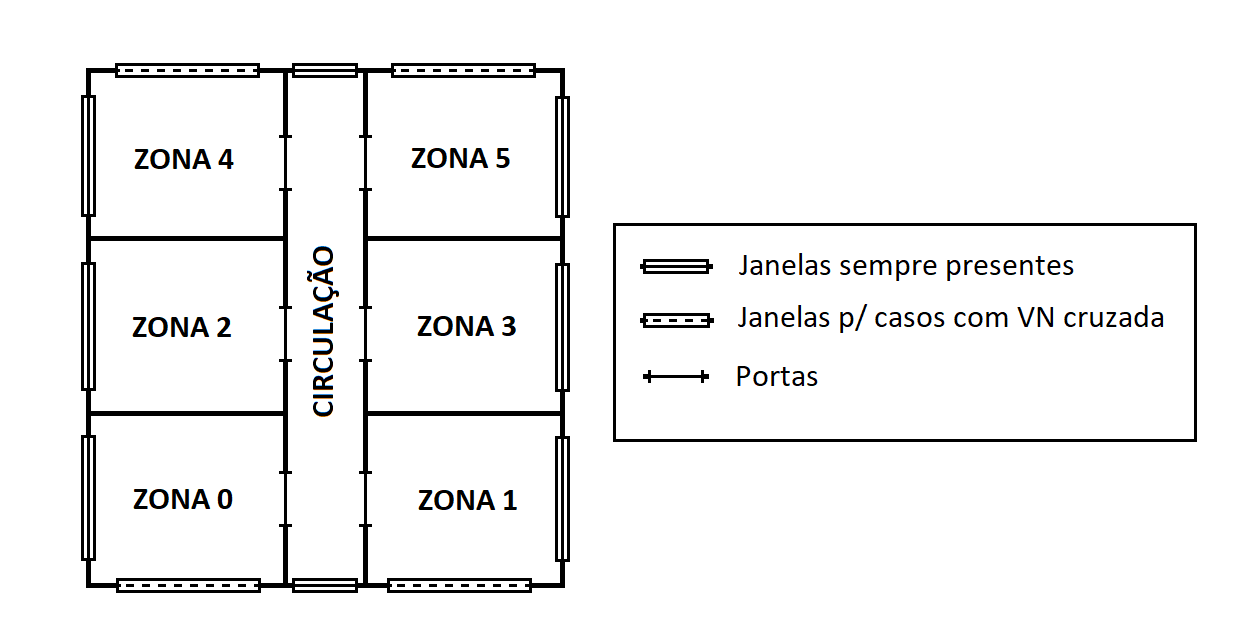
\includegraphics[width=.8\linewidth]{img/croqui_07-11.png}
	\label{fig:croqui}
\end{figure}


A partir da tipologia base, foi possível definir diferentes proporções geométricas, levando-se em consideração a largura e profundidade da edificação, assim como o pé-direito. Também foram parametrizadas a altura do pavimento e a orientação solar da edificação.
Devido a limitações na obtenção dos \acrfull{cp} para as faces externas da edificação, as edificações foram modeladas com pavimentos de forma retangular.

A parametrização nas propriedades termofísicas das paredes e vidros permitiu a consideração de diferentes materiais construtivos, possibilitando a descrição de uma quantidade significativa do universo de casos aplicáveis às edificações de escritórios consideradas. %Foram parametrizadas a transmitância térmica, capacidade térmica e absortância.

Para considerar o uso de \acrfull{vn}, é fundamental a modelagem das trocas de ar nos escritórios. A modelagem da \acrshort{vn} nas simulações foi realizada com os objetos do \acrfull{afn} do EnergyPlus \cite{EnergyPlus2018}.
Para possibilitar trocas de ar, elementos de ligação do \acrshort{afn} foram modelados em todas as zonas térmicas.
Todas as aberturas foram modeladas utilizando-se o objeto \textit{AirflowNetwork:MultiZone:Component:DetailedOpening}.
Cada sala foi modelada com uma porta, voltada para a circulação.
Na circulação, além das portas das salas, duas janelas foram modeladas, uma em cada extremidade. 
Salas com apenas uma fachada foram modeladas com uma janela; salas com duas fachadas foram modeladas com uma ou duas janelas. Isso possibilitou explorar casos com diferentes configurações de exposição das superfícies, considerando-se \acrshort{vn} unilateral e cruzada.		
As dimensões das janelas das salas foram parametrizadas de acordo com o \acrfull{paf}, permitindo diferentes frações de abertura para representar diferentes modelos de janela encontrados nas edificações de escritórios existentes no banco de dados.
%Além da área da abertura ter influência direta nas trocas de ar das zonas, a altura também pode ter influência devido à força de empuxo causada pelas diferenças de densidade do ar. Devido a isso, a altura da janela também foi parametrizada.
%		Para o vidro das janelas considerou-se diferentes valores para o fator solar.
%		\subsection{Ventilação natural no modelo preliminar}
O controle das janelas foi estabelecido de maneira independente para cada zona térmica, pela diferença de temperatura entre o ar externo e o ar da zona.
As trocas de ar nas portas foram modeladas apenas por frestas, por considerar-se que portas de escritórios não ficam abertas normalmente.  % MELHORAR!!!
Os coeficientes de pressão nos nós externos à edificação foram definidos através da base de dados da \acrlong{tpu} \cite{TPU2018}, e para cada janela foi utilizado o valor médio dos pontos disponíveis para sua área na fachada. No o exemplo da Figura \ref{fig:tpuwindows}, considerando-se uma edificação com proporções B:L:H, e um pavimento na altura h, o \acrshort{cp} da janela A seria igual à média dos valores disponíveis para os pontos vermelhos, o \acrshort{cp} da janela B seria igual à média dos valores dos pontos verdes, e assim por diante.
%		A altura dos pontos a serem utilizadas foi escolhida de acordo com a altura definida para o pavimento simulado e  a altura do pédireito em relação às proporções do edifício.

\begin{figure}[h]
	\centering
	\caption{Exemplo de como os $C_p$ foram considerados}
	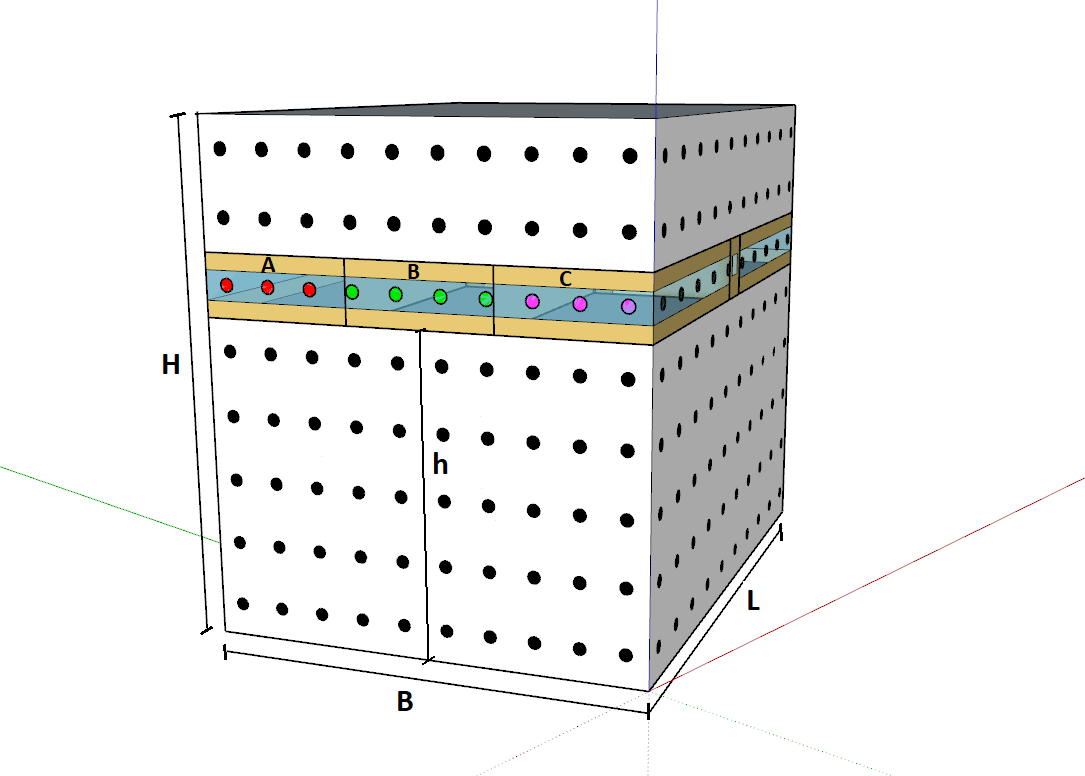
\includegraphics[width=.8\linewidth]{img/ex_TPU_h.png}
	\label{fig:tpuwindows}
\end{figure}


\subsection{Simulação simplificada}

Nesta etapa do método, buscou-se simplificar o modelo de escritório desenvolvido no EnergyPlus, atentando-se às limitações relacionadas à simplificação do modelo.
O objetivo de gerar um metamodelo por meio de \acrfull{ann} para se obter o \acrshort{ehf} faz com que se busque parametrizar ao máximo as simulações no EnergyPlus.
Essa parametrização pode facilitar o desenvolvimento de amostras para a pesquisa, assim como garantir uma relação mais direta dos parâmetros de entrada com os dados de saída. 
As seguintes simplificações foram consideradas, e serão explicadas nesta seção:

\begin{itemize}
	\item cálculo do \acrshort{cp} através do \acrlong{ma}, em vez dos valores obtidos por medições em túnel de vento pela \acrshort{tpu};
	\item representação dos materiais da envoltória através de duas camadas: uma camada representando a capacidade térmica, e uma camada para regular a transmitância;  %(concreto)  (objeto Material:NoMass)
	\item modelagem da zona que representa apenas um escritório, sem modelar as demais zonas térmicas da edificação. Para isso, são definidas as condições de contorno relacionadas às faces da zona correspondentes a paredes adjacentes à edificação;
	\item definição de um coeficiente de vazão mássica de ar relacionado à infiltração de ar pela porta, e do valor do \acrshort{cp} relacionado a essa porta, que no modelo de uma zona está voltada para o ambiente externo, e não para a circulação.
\end{itemize}

O impacto nos resultados das simulações foram verificados para cada uma das simplificações mencionadas, a partir da análise de diversos casos amostrados pelo método de amostragem do hipercubo latino (LHS). O tamanho das amostras foi definido em relação ao tempo disponível para executar as simulações.
Finalmente, foi definida a forma mais adequada de se simplificar o modelo, assim como a margem de erro que espera-se encontrar ao assumir tais simplificações.
A seguir, cada uma dessas etapas é descrita.

\subsection*{Cálculo do coeficiente de pressão pelo método analítico}

O EnergyPlus, através do \acrshort{afn}, possui uma opção para calcular automaticamente os \acrshort{cp} para as simulações.
Quando essa opção é escolhida o programa gera apenas um \acrshort{cp} por fachada da edificação, e os valores podem ser obtidos por dois algorítimos diferentes: no caso de edificações altas (\textit{highrise}), utiliza-se o modelo de \citeonline{Atkins}; no caso de edificações baixas (\textit{lowrise}), utiliza-se o modelo de \citeonline{Swami1988}.
Enquanto que pelo \acrlong{ma} os \acrshort{cp} podem ser obtidos para quaisquer razões entre as dimensões das fachadas da edificação, os valores medidos em túnel de vento pela \acrshort{tpu} são fornecidos para edificações com proporções entre largura, profundida e altura específicas.
Os valores de \acrshort{cp} para o tipo de edificação abordada neste estudo são disponibilizados pela \acrshort{tpu} para 25 geometrias diferentes, das quais 13 são para edificações \textit{highrise}, e 12 são para edificações \textit{lowrise}.

Para verificar o quanto a fonte escolhida na definição dos \acrshort{cp} influencia nos resultados das simulações, inicialmente verificou-se as diferenças entre os valores dos \acrshort{cp} das medições em túnel de vento (fornecidos pela \acrshort{tpu}), e os valores dos \acrshort{cp} obtidos pelo \acrlong{ma} (algorítimos do EnergyPlus). Para cada uma das 25 geometrias disponíveis, calculou-se a diferença entre os \acrshort{cp}, de acordo com a Equação \ref{eq:Cpdiff}. 
Geometrias definidas como \textit{highrise} pela \acrshort{tpu} foram comparadas utilizando-se o \acrlong{ma} de \citeonline{Atkins}, enquanto que geometrias definidas como \textit{lowrise} pela \acrshort{tpu} foram comparadas utilizando o \acrlong{ma} de \citeonline{Swami1988}.

\begin{equation}
\label{eq:Cpdiff}
RMSE_{Cp} = \sqrt{\frac{\sum_{i=1}^{4}{\sum_{j=0}^{11}}{\sum_{k=0}^{N_d}{(\overline{Cp}^{TPU}_{f_i,\alpha_j,p_k} - Cp^{MA}_{f_i,\alpha_j}})^2}}{48}}
\end{equation}

Onde:

\gls{rmsecp} é igual ao \acrshort{rmse} das diferenças entre os valores dos \acrshort{cp} obtidos pela base da \acrshort{tpu} e obtidos pelo \acrlong{ma};

\gls{meancptpu} é igual ao valor do \acrshort{cp} disponibilizado pela base de dados da \acrshort{tpu} para a fachada $i$ de uma edificação, para o ângulo de incidência do vento igual a $\alpha_j$, no ponto $k$;

\gls{cpma} é igual ao \acrshort{cp} calculado pelo \acrlong{ma} para a fachada de uma edificação com proporções iguais às da fachada $i$, para o ângulo de incidência do vento igual a $\alpha_j$;

\gls{fi} é a fachada $i$ da edificação avaliada;

\gls{alphaj} é o ângulo de incidência do vento  sobre a fachada, em graus, e tem valor igual a $30 \cdot j$;

\gls{nd} é o número de pontos de \acrshort{cp}` disponibilizados na fachada do edifício.	
%		$\alpha_j$ é o ângulo de incidência do vento considerado sobre a fachada, que varia de 0 a 330 graus, com intervalos de 30 graus;
\\

%		Cada \acrshort{cp} médio ($Cp_{TPU,i,j}$), medido pela \acrshort{tpu} em um ponto $j$ de uma fachada $i$, teve um \acrshort{cp} correspondente calculado pelo método analítico ($Cp_{ANALITICO, i}$), para a mesma fachada $i$. Essa subtração foi efetuada para os diferentes ângulos ($\alpha$) disponíveis na base da \acrshort{tpu}.
%		As diferenças entre os valores dos \acrshort{cp} foram calculadas obtendo-se o \acrshort{cp} pelo método analítico para cada fachada, de cada geometria disponível pela \acrshort{tpu}, e subtraindo-se o valor do \acrshort{cp} calculado pelos valores disponibilizados pela base da \acrshort{tpu} para a sua fachada correspondente (Equação \ref{eq:Cpdiff}).

A partir dessas diferenças entre os valores dos \acrshort{cp}, escolheu-se a geometria com o maior  \gls{rmsecp} como modelo base na análise da influência nos resultados das simulações no EnergyPlus.
Esta análise foi conduzida gerando-se uma amostra de 1.000 casos pelo LHS.
Os parâmetros variados e seus limites mínimos e máximos foram definidos pela metodologia do item \ref{subsec:par}, com exceção da razão entre a largura e profundidade das zonas e a altura do pavimento em relação ao solo.
A razão entre a largura e profundidade das zonas teve que ser alterada de acordo com a variação da área das salas, para se ajustar à geometria da edificação definida como modelo base da análise.
A altura do pavimento em relação ao solo também foi limitada pelas proporções da geometria escolhida para o modelo base.
Vale destacar que a base da \acrshort{tpu} permite a obtenção de diferentes \acrshort{cp} para diferentes janelas de uma mesma fachada, enquanto que nas simulações baseadas no \acrlong{ma}, utiliza-se apenas um valor de \acrshort{cp} por fachada, devido à limitação do método. 
Para cada caso da amostra gerada, foram simulados um modelo com \acrshort{cp} baseados no \acrlong{ma}, e um modelo com \acrshort{cp} baseados na base da \acrshort{tpu} (túnel de vento).
Assim, as médias anuais das \acrfull{ach} e a \acrshort{ehf} foram comparadas entre as simulações.
%		com \acrshort{cp} medidos em túnel de vento pela \acrshort{tpu}, e simulações com \acrshort{cp} obtidos pelos métodos analíticos padrão do EnergyPlus.

%		Para cada uma dessas geometrias disponíveis, valores de \acrshort{cp} são disponibilizados para diversos pontos na fachada da edificação, de acordo com a Figura \ref{fig:tpupoints}.
%		
%		\begin{figure}[h]
%			\centering
%			\caption{Exemplo do posicionamento dos pontos com valores de \acrshort{cp} na fachada}
%			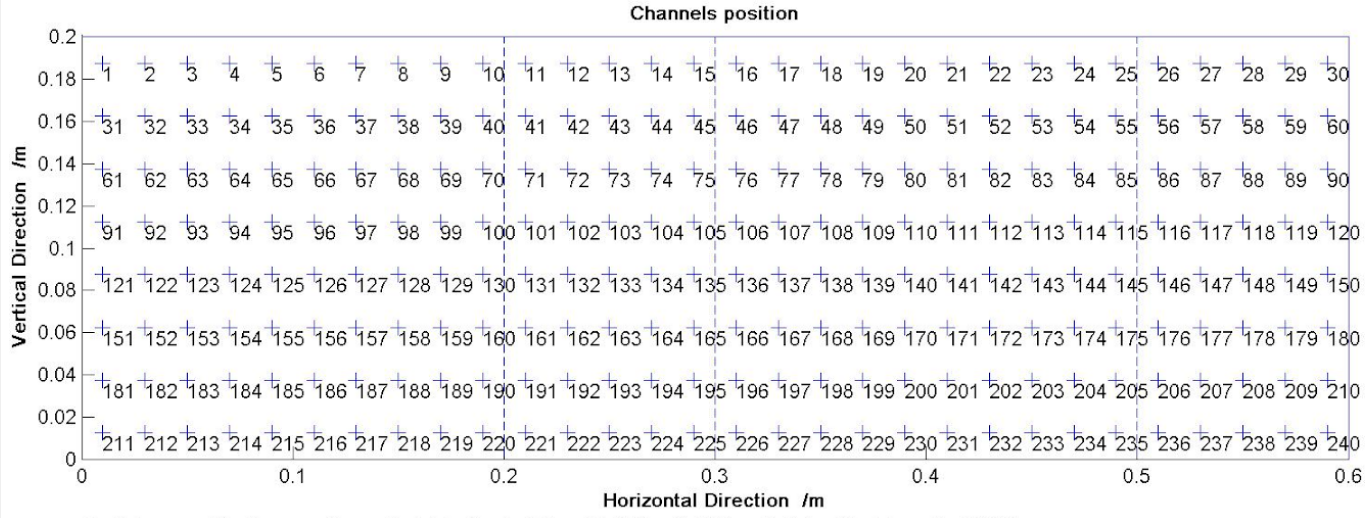
\includegraphics[width=\figsize\linewidth]{img/tpu_points.png}
%			\label{fig:tpupoints}
%			\begin{flushleft}
%				Fonte: \citeauthoronline{TPU2018} \cite{TPU2018}, adaptado pelo autor.
%			\end{flushleft}
%		\end{figure}					

\subsection*{Representação da envoltória com duas camadas}

Para possibilitar a parametrização contínua e independente das propriedades termofísicas da envoltória, considerou-se a utilização de uma parede com propriedades equivalentes, modelada com uma camada de concreto, para representar a capacidade térmica, e uma camada modelada com o objeto \textit{Material:NoMass}, para regular a transmitância (Figura \ref{fig:parede_eq}).

\begin{figure}[h]
	\centering
	\caption{Parede equivalente}
	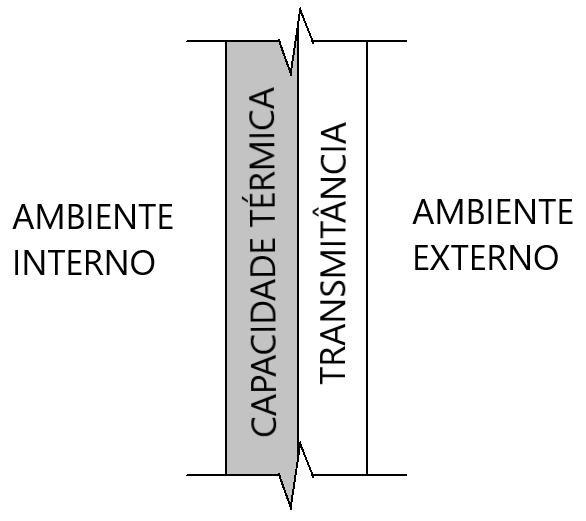
\includegraphics[width=.3\linewidth]{img/parede_eq2.png}
	\label{fig:parede_eq}
\end{figure}

A validação da modelagem simplificada da parede foi realizada para dois tipos de paredes referência (uma leve, outra pesada):

\begin{itemize}
	%			\item parede de concreto;
	\item parede de gesso com lã de rocha (leve);
	\item parede de alvenaria e reboco (pesada).
\end{itemize}

Como a modelagem da parede de alvenaria possui uma camada de ar no meio da parede, avaliou-se a possibilidade de considerar apenas a metade interna desta parede referência para definir a capacidade térmica de sua parede equivalente. Essa consideração parte do pressuposto de que a camada interna de ar faz com que a inércia térmica da metade exterior da parede não influencie consideravelmente a zona térmica analisada.

Para validar essa simplificação, gerou-se uma amostra utilizando LHS, com 100 casos.
Os parâmetros variados e seus limites mínimos e máximos foram definidos pela metodologia do item \ref{subsec:par}, com exceção da transmitância e capacidade térmica da parede.  % os parâmetros relacionados com a propriedades termofísicas da parede.	% e a absortância????
%		O modelo preliminar sofreu variação dos seguintes parâmetros: área, razão entre largura e profundidade da zona, pé-direito, azimute, absortância, \acrshort{paf}, taxa de ocupação. Os demais parâmtros foram fixados de acordo com a Tabela \ref{table:paramfix}.
Cada caso da amostra foi simulado com os dois tipos de paredes diferentes, e suas paredes equivalentes. No caso da parede de alvenaria, dois modelos de parede equivalente foram desenvolvidos: considerando o valor total da capacidade térmica da parede, e considerado apenas metade do valor da capacidade térmica.
A partir dos resultados, observou-se a diferença média entre as temperaturas operativas das zonas simuladas com as paredes referências em relação às simulações com as respectivas paredes equivalentes. O mesmo foi realizado comparando-se o \acrshort{ehf}.

\subsection*{Condição de contorno das paredes adjacentes à edificação}

Simular apenas uma zona térmica, em vez de um edifício inteiro, ou um pavimento com diversas zonas, possibilita a simulação de casos diversos em menor tempo.
Essa consideração facilita a parametrização do modelo, e pode oferecer resultados satisfatórios se for adequadamente implementada.
A partir dessa premissa, foi desenvolvido um modelo com apenas uma zona térmica (Figura \ref{fig:singlezone}).

\begin{figure}[h]
	\centering
	\caption{Modelo de uma zona}
	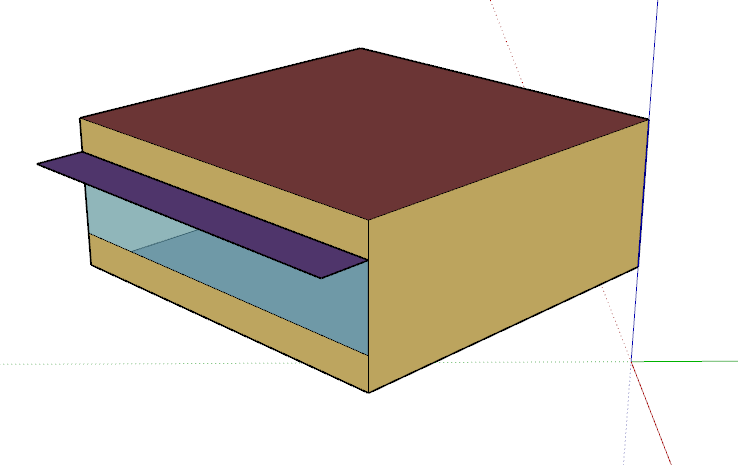
\includegraphics[width=\figsize\linewidth]{img/model.PNG}
	\label{fig:singlezone}
\end{figure}

Para modelar essa zona, considerou-se as paredes correspondentes a superfícies voltadas para outros escritórios como adiabáticas (sem trocas de calor). A superfície que representa a parede voltada para a circulação foi avaliada com duas condições de contorno: 1) como adiabática, e 2) como \textit{outdoors}, sem incidência de vento ou sol (Figura \ref{fig:adiabatic_outdoors}).	
A consideração do uso da condição \textit{outdoors} foi realizado pela hipótese de que, sem a radiação solar direta e sem o aumento de convecção causada pelo vento, a temperatura do ar da zona da circulação (por não ter cargas internas consideráveis) poderia se manter mais próxima à temperatura do ar externo do que às das zonas das salas de escritórios.

\begin{figure}[h]
	\centering
	\caption{Modelagem com parede adiabática e \textit{outdoors}}
	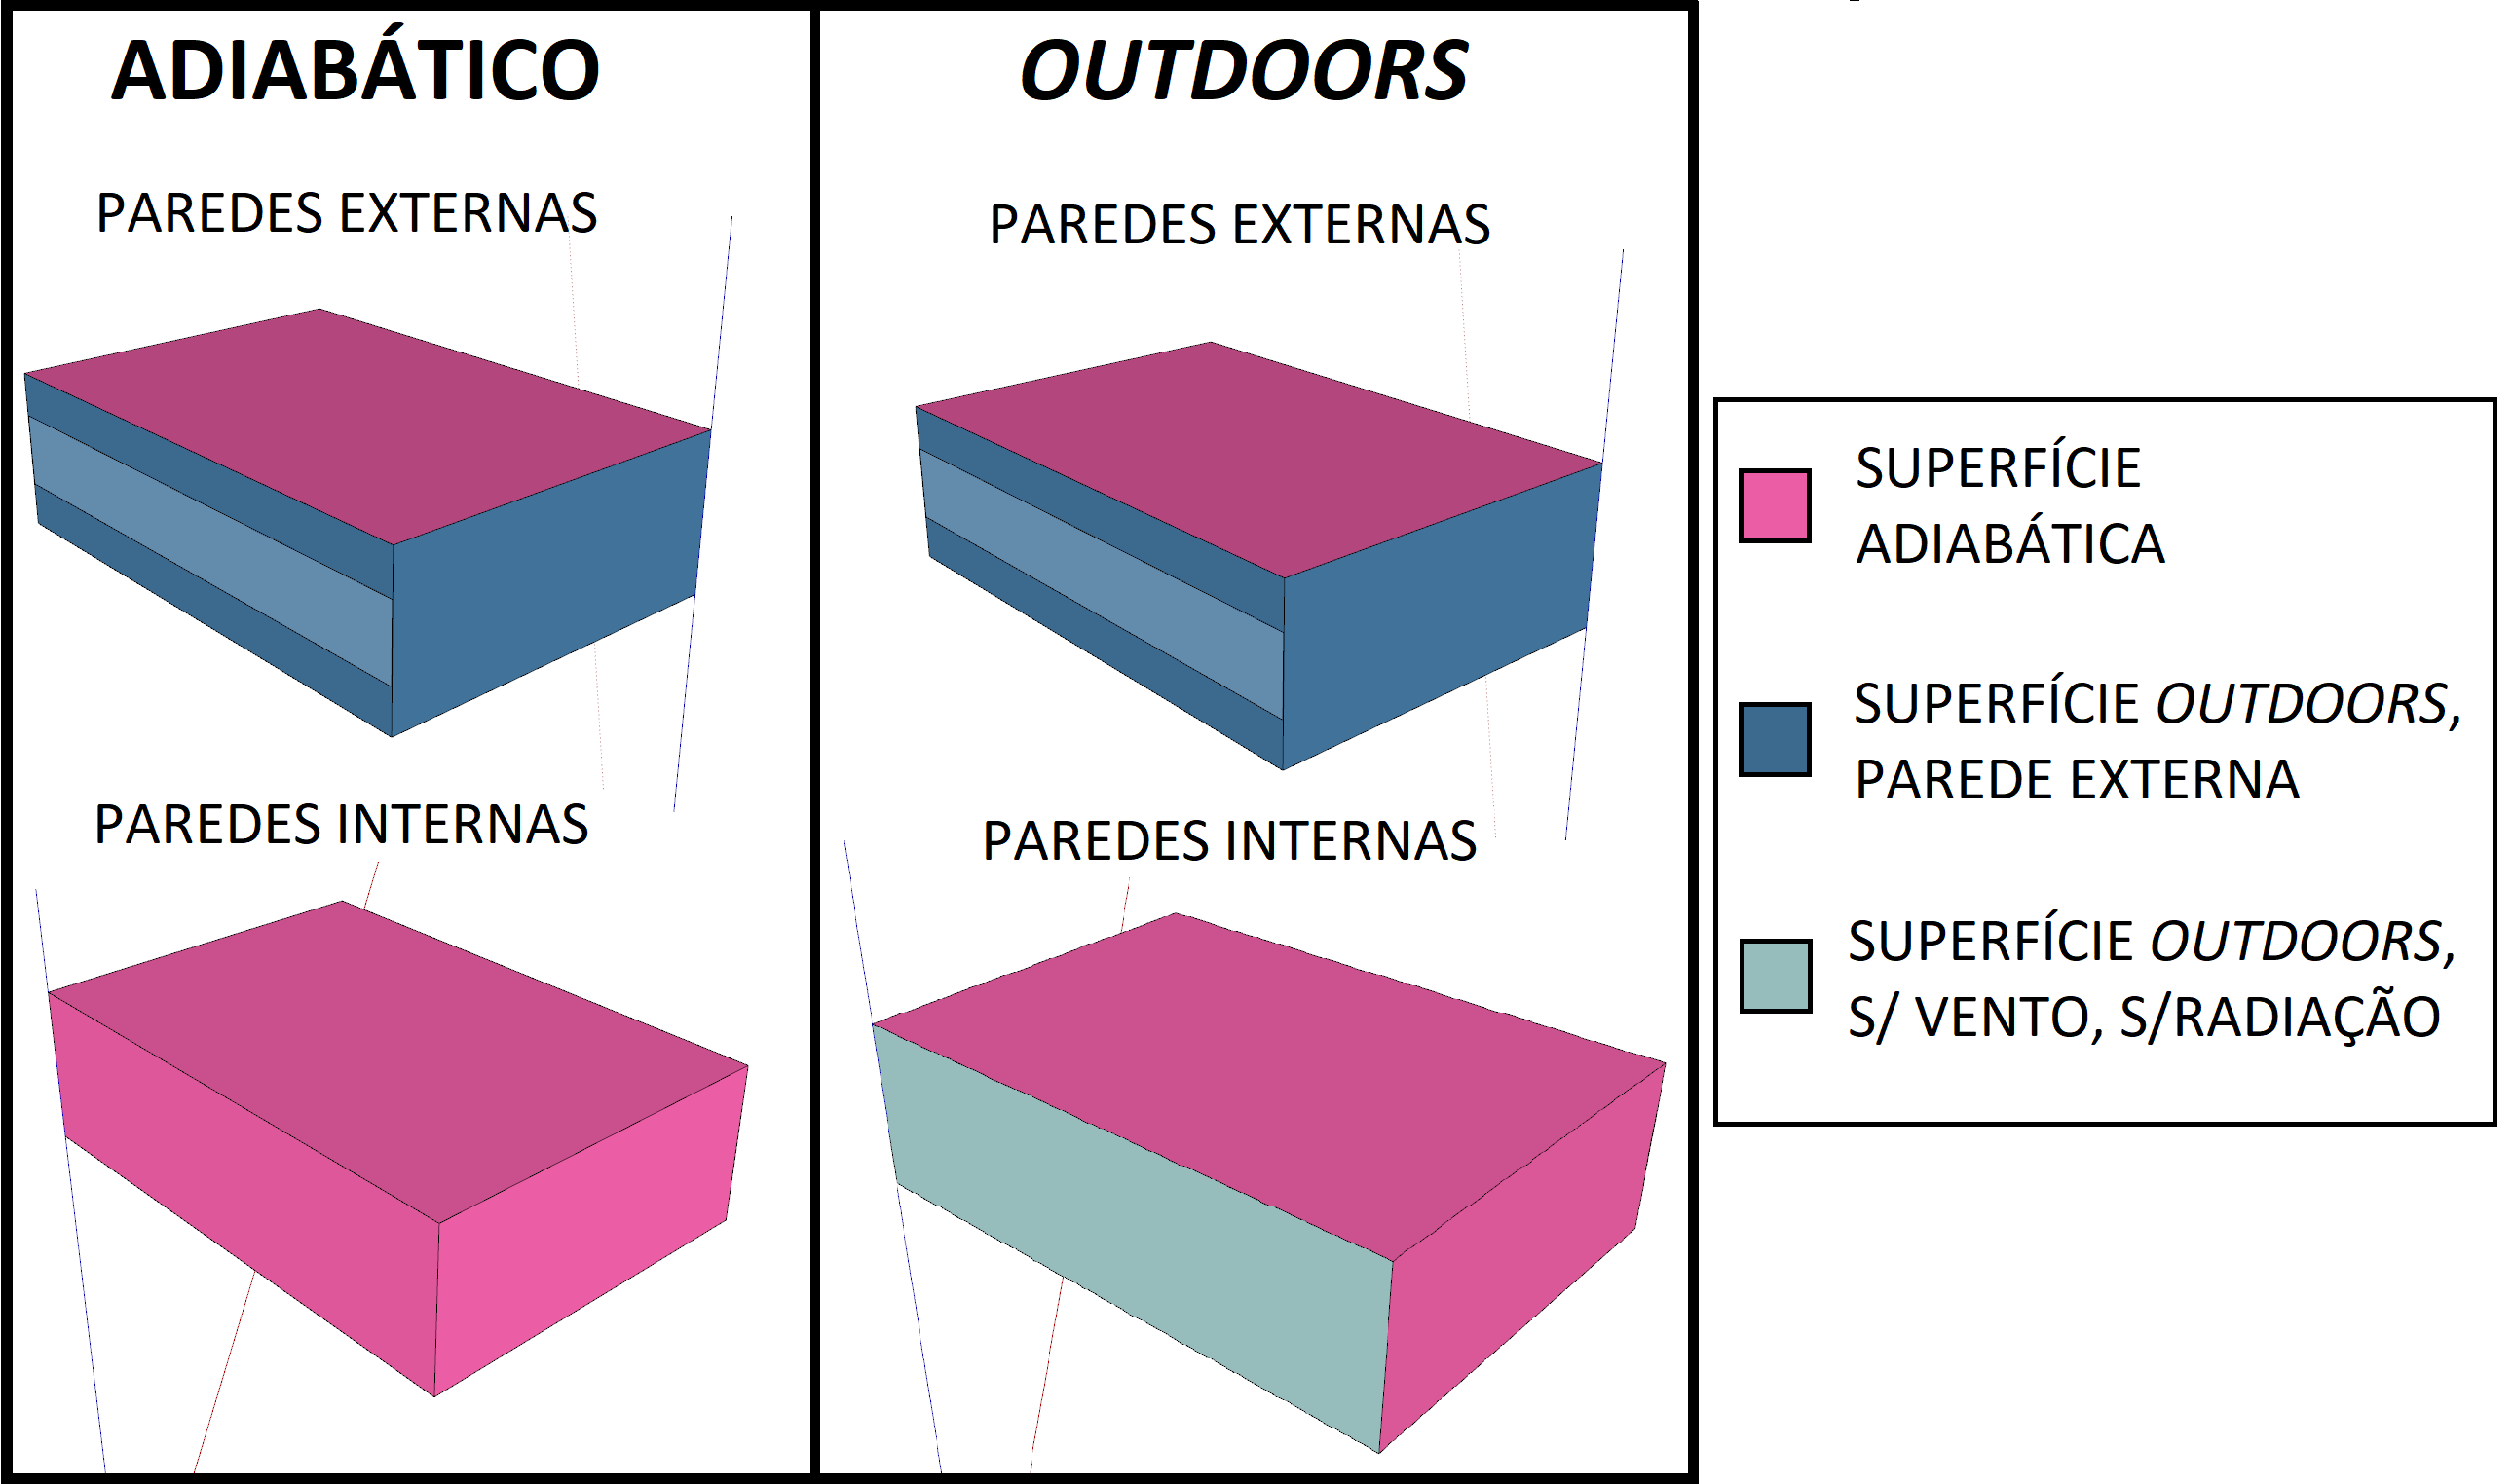
\includegraphics[width=.7\linewidth]{img/adiabatic_outdoors2.png}
	\label{fig:adiabatic_outdoors}
\end{figure}


A modelagem da \acrlong{vn} sofre um impacto significativo quando o escritório é modelado como apenas uma zona térmica.
Esse impacto é devido à forma como a rede de fluxo de ar é distribuída. No caso do modelo detalhado, a porta é voltada para a circulação, enquanto que no caso de uma única zona térmica, a porta desta zona é voltada para o ambiente externo. 
Além disso, não é possível modelar uma porta em uma parede adiabática. Para não deixar a diferença na \acrlong{vn} influenciar as análises comparativas entre as simulações, a \acrlong{vn} não foi modelada para esta etapa.
Em vez disso, as simulações foram desenvolvidas com uma taxa de infiltração de ar constante durante a ocupação. O valor escolhido para a taxa de renovação de ar foi igual ao valor médio do \acrshort{ach} obtido na etapa da comparação entre os \acrshort{cp}, que é igual a 30 \acrshort{ach}.

A amostra gerada pelo LHS nesta etapa foi de 100 casos.
Os parâmetros variados e seus limites mínimos e máximos foram definidos pela metodologia do item \ref{subsec:par}.
Para cada caso gerado pelo LHS, além da simulação detalhada, seis modelos de uma zona foram simulados, correspondendo a cada uma das zonas do modelo detalhado.
Para validar o uso de diferentes condições de contorno, comparou-se os resultados de \acrshort{ehf} e temperaturas operativas das simulações de uma zona térmica com os resultados obtidos para as zonas térmicas das simulações detalhadas.
A condição de contorno com menores diferenças médias, de temperatura operativa e \acrshort{ehf}, foi escolhida para se conduzir as simulações simplificadas.

\subsection*{Modelagem da ventilação natural na simulação simplificada}

A modelagem da \acrlong{vn} na simulação simplificada deve ser adaptada para se ter resultados correspondentes ao esperado em relação à simulação detalhada, pois enquanto a rede de fluxo de ar na simulação detalhada é modelada de acordo com a Figura \ref{fig:AFN_ref}, na simulação simplificada essa rede é modelada de acordo com a Figura \ref{fig:AFN_sz}.	

\vspace{20pt}
\begin{figure}[h]
	\centering
	\caption{Rede de fluxo de ar na simulação detalhada}
	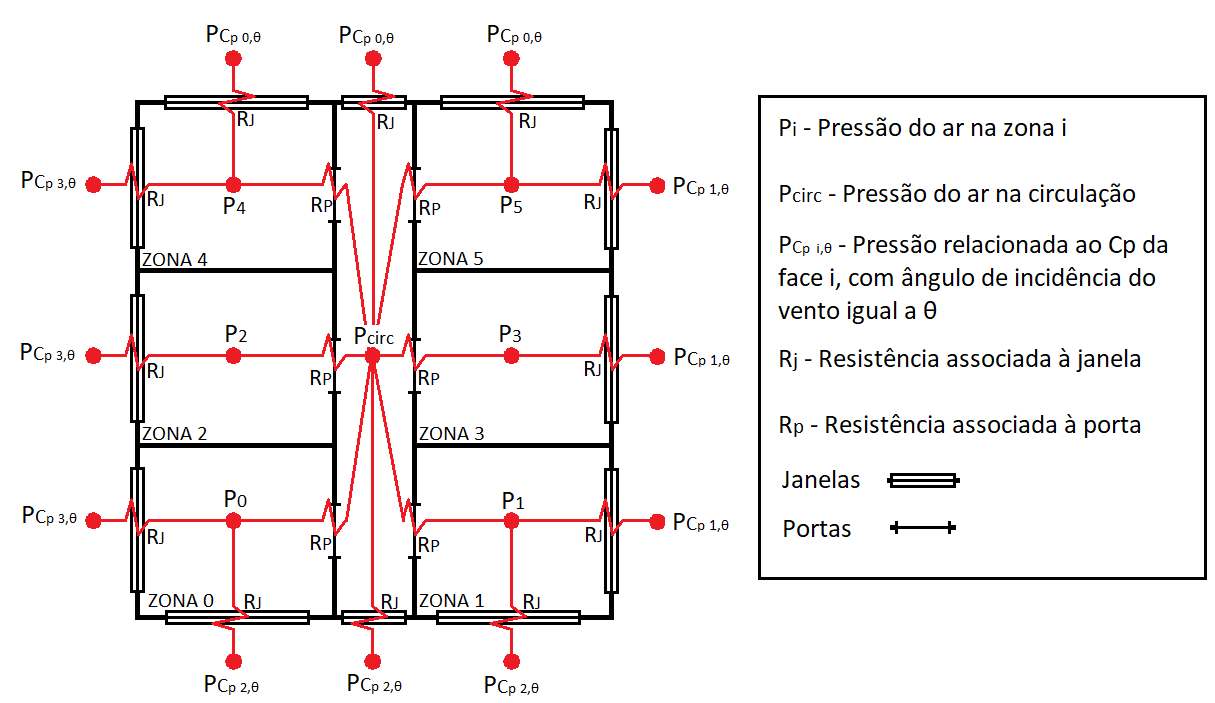
\includegraphics[width=1\linewidth]{img/AFN_ref2.png}
	\label{fig:AFN_ref}
\end{figure}	

\begin{figure}[h]
	\centering
	\caption{Rede de fluxo de ar na simulação simplificada}
	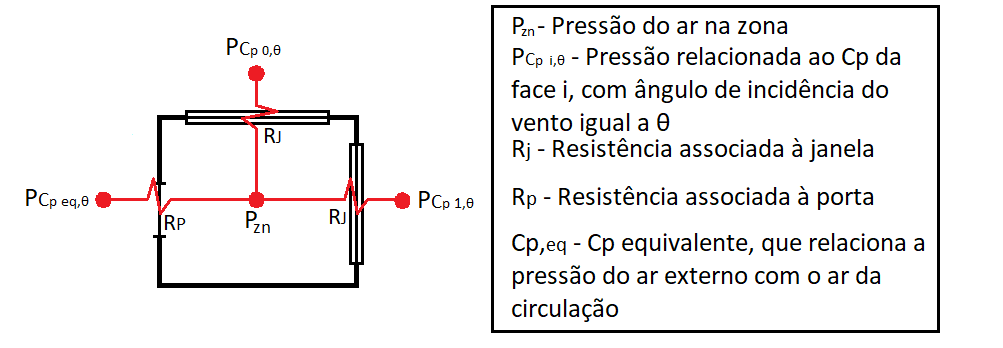
\includegraphics[width=.8\linewidth]{img/AFN_sz2.png}
	\label{fig:AFN_sz}
\end{figure}
\newpage
A proposta para contornar esse problema foi desenvolvida a partir da hipótese de que, na simulação simplificada, seria possível criar um \acrshort{cp} associado à porta ($Cp_{eq}$), capaz de descrever as diferenças de pressão de ar entre a circulação e a sala.  % , para cada ângulo de vento.

Quando o objeto \textit{AirflowNetwork:MultiZone:Component: DetailedOpening} é utilizado, o cálculo do fluxo de ar entre dois pontos é feito pela Equação \ref{eq:AFEDOP_opened}, se a porta/janela está aberta, ou pela Equação \ref{eq:AFEDOP_closed}, que é utilizada para calcular a infiltração de ar quando a abertura está fechada.

\begin{equation}
\label{eq:AFEDOP_opened}
\dot{m}_{i,j} = C_d \Theta 	\int_{z=0}^{z=H} \sqrt{2 \rho (P_{i(z)} - P_{j(z)})} W d_z 
\end{equation}

\begin{equation}
\label{eq:AFEDOP_closed}
\begin{split}
\dot{n}_{i,j} = C_Q [2\int_{z=0}^{z=H} {(P_{i(z)} - P_{j(z)})}^{exp} d_z + \\ W{(P_{i(0)} - P_{j(0)})}^{exp} + W{(P_{i(H)} - P_{j(H)})}^{exp}]
\end{split}
\end{equation}

Onde:

\gls{m} é o fluxo de ar entre os pontos $i$ e $j$, quando a porta/janela está aberta (kg/s);

\gls{cdd} é o coeficiente de descarga da abertura ($-$);

\gls{theta} é a fração de abertura ($-$);

\gls{height} é a altura da abertura ($m$);

\gls{piz} é a pressão de ar no ponto $i$, altura $z$ ($Pa$);

\gls{width} é a largura da abertura ($m$);

\gls{n} é o fluxo de ar entre os pontos $i$ e $j$, quando a porta/janela está fechada ($kg/s$);

\gls{cqq} é o coeficiente de vazão mássica de ar da abertura ($-$);

\gls{exp} é o expoente de vazão mássica de ar ($-$).
\\

As seguintes condições de contorno foram estabelecidas para facilitar o cálculo do $Cp_{eq}$:
\begin{itemize}			 
	\item o valor do $exp$ foi definido como 0,5;
	\item o valor de $\rho$ foi definido sempre como 1,200 kg/m$^3$;
	\item os fluxos de ar foram considerados como unidimensionais, portanto os valores de $P$ não variaram com o a altura ($z$);
	\item O valor do $Cp_{eq}$ foi definido assumindo-se que as janelas estariam com sua máxima fração de abertura ($\Theta$).
\end{itemize}

Em cada \textit{timestep}, a soma dos fluxos de ar que entram e saem de uma zona $i$ é igual a zero. Assumindo-se as condições de contorno descritas, a pressão de ar em cada zona térmica pode ser estimada pela Equação \ref{eq:P}. Dessa forma é possível encontrar a relação entre as pressões de ar de todas as zonas da simulação detalhada.

\begin{equation}\label{eq:P}
%\resizebox{\linewidth}{!}{
\begin{split}
P_{zn} = \frac{\sum_{i=1}^{N_P}{P_{i} (C_q L_i)^2} +  %\\
	\sum_{j=1}^{N_J}{(P_{d} C_{p,j} + P_{\infty}) 2 \rho (C_{d} \Theta_j A_j)^2 }}
{\sum_{i=1}^{N_P}{(C_q L_i)^2} +  %\\
	\sum_{j=1}^{N_J}{2 \rho (C_{d} \Theta_j A_j)^2 }}
\end{split}
%}
\end{equation}

Onde:

\gls{pzn} é a pressão do ar na zona analisada ($Pa$);

\gls{np} é igual ao número de portas que se conectam à zona ($-$);

\gls{pi} é a pressão de ar na zona ligada pela porta $i$ ($Pa$);

\gls{li} é igual ao perímetro da porta $i$ ($m$);

\gls{nj} é igual ao número de janelas que se conectam à zona ($-$);

\gls{pd} é a pressão dinâmica do ar ($Pa$);

\gls{p0} é a pressão estática do ar no ambiente externo ($Pa$);

\gls{cpj} é o \acrshort{cp} na superfície da janela $j$ ($-$);

\gls{area} é igual à área da janela $j$ ($m^2$).
\\

Finalmente, os \acrshort{cp} equivalentes (\acrshort{cpeq}) foram definidos calculando-se a relação entre a pressão de ar na zona da circulação e a pressão do ar no ambiente externo, para cada direção angular do vento, de acordo com a Equação \ref{eq:Cpeq}.

\begin{equation}\label{eq:Cpeq}
Cp_{eq,\alpha} = \frac{P_{circ}-P_{\infty}}{P_{d}}
\end{equation}

Onde:

$P_{circ}$ é a pressão de ar na circulação;

$Cp_{eq,\alpha}$ é igual ao \acrshort{cp} equivalente na abertura da porta, para um ângulo de vento $\alpha$.
\\

Outra limitação relacionada à \acrshort{vn} na simulação simplificada é o fato de que o \acrshort{afn} do EnergyPlus não permite modelar aberturas ou qualquer tipo de infiltração de ar em superfícies adiabáticas. Para contornar esse problema, no caso de se modelar uma parede voltada para a circulação como adiabática, é possível associar a infiltração referente à porta a uma outra superfície da zona.  %  que esteja voltada para o ambiente externo 
Isso se faz possível no momento em que se calcula diretamente os \acrfull{cp} dos nós relacionados às aberturas da zona térmica.
Desta forma define-se o \acrshort{cp} para uma superfície (seja janela ou parede), considerando-se qualquer orientação desejada, e não necessariamente a orientação definida para esta superfície pela geometria do modelo.		
A modelagem do fluxo de ar pelas portas dos escritórios nas simulações simplificadas foi desenvolvida com o objeto \textit{AirflowNetwork:MultiZone:Surface:Crack}. O motivo para se utilizar este objeto é porque este é um objeto que pode ser associado a qualquer tipo de superfície. Portanto, o objeto do \textit{crack} foi associado sempre à parede externa oposta à parede que estaria voltada para a circulação, como apresentado na Figura \ref{fig:AFN_crack}.

Devido a essas considerações, a validação nesta etapa foi conduzida para duas condições: utilizando-se o \acrshort{cp} calculado diretamente pelo método analítico, e utilizando-se o \acrfull{cpeq}.		
Estas análises foram conduzidas considerando-se diferentes valores de coeficiente de vazão mássica de ar para o \textit{crack}, para ajustar o valor mais adequado à taxa de infiltração que se obtém no modelo detalhado. Os valores considerados foram: 0,005; 0,010; 0,100; e 0,200 kg/s em 1 Pa.
Uma amostra de 200 casos foi gerada por LHS.
Os parâmetros variados e seus limites mínimos e máximos foram definidos pela metodologia do item \ref{subsec:par}.
Para cada caso, gerou-se uma simulação detalhada, mais 120 simulações simplificadas. Essas 120 simulações simplificadas devem-se à consideração dos dois métodos para se obter os \acrshort{cp}, mais os dez valores de coeficiente de vazão mássica de ar analisados, avaliados para as seis zonas térmicas do modelo detalhado. 
Para escolher a configuração mais adequada entre os métodos de obtenção do \acrshort{cp} e o coeficiente de vazão mássica de ar, as comparações foram efetuadas observando-se os resultados das médias anuais de \acrshort{ach} e \acrshort{ehf}.
%A escolha da melhor configuração observando-se dois indicadores simultaneamente foi possível através de uma análise de eficiência de Pareto.
%Como as taxas de infiltração são influenciadas pela temperatura do ar, as comparações com os modelos detalhados foram feitas considerando-se diferentes faixas de temperatura.

\begin{figure}[H]
	\centering
	\caption{Solução para infiltração de ar entre a zona e a circulação}
	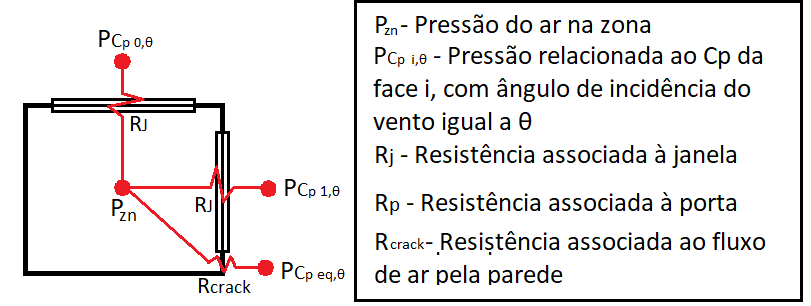
\includegraphics[width=.8\linewidth]{img/AFN_crack2.png}
	\label{fig:AFN_crack}
\end{figure}
%\vspace{-100pt}

\section{Análise de sensibilidade}

Após definir como seriam desenvolvidos os modelos para as simulações simplificadas, uma \acrfull{as} foi aplicada. Através da \acrshort{as}, a influência dos diferentes dados de entrada variados nas simulações foi avaliada. Com base nos resultados da \acrshort{as}, parâmetros não relevantes nos resultados de temperatura operativa e, consequentemente, \acrfull{ehf}, foram determinados com valores fixos. Desta forma, o metamodelo foi desenvolvido considerando-se apenas parâmetros com influência expressiva nos dados de saída desejados.

O método de \citeauthoronline{Sobol1993} \cite{Sobol1993} foi utilizado para a \acrshort{as}, pois permite a identificação de parâmetros influentes, mesmo para casos onde a relação entre as entradas e saídas dos modelos são não-monotônicas e apresentam efeitos colineares.

A \acrshort{as} foi aplicada por meio de programação, utilizando-se a biblioteca \textit{SALib} \cite{Herman2017}, escrita na linguagem \citeonline{Python}, versão 3.
Os casos simulados para conduzir a \acrshort{as} foram amostrados pelo método de amostragem específico da \acrshort{as} de Sobol, pelo qual gerou-se uma amostra de 155.648 casos.
Os parâmetros variados e seus limites mínimos e máximos foram definidos pela metodologia do item \ref{subsec:par}. 
%, que gera uma sequência quasi-randômica de baixa discrepância.é uma é feita a partir de uma amostra desenevolvida específica para essa análise é definida pelo próprio método, pela qual gerou-se 99.978 casos.		
A partir dos dados de entrada de cada caso, e dos valores das médias anuais de \acrshort{ach}, médias anuais de temperatura operativa, e \acrshort{ehf} resultantes das simulações termoenergéticas, obteve-se índices de sensibilidade para análise de primeira ordem, segunda ordem, e efeitos totais.
%\vspace{50pt}
\newpage

\section{Desenvolvimento do metamodelo}

O metamodelo foi desenvolvido por meio de \acrfull{ann}, utilizando a biblioteca \textit{TensorFlow} \cite{tensorflow2015}, disponibilizada para \citeonline{Python}.
A maneira como se descreve as variáveis de entrada dos modelos simulados para o metamodelo a ser desenvolvido pode influenciar na sua precisão e na representação adequada dos fenômenos termofísicos.
Portanto, no processo de definição das variáveis de entrada do metamodelo, busca-se a melhor forma de descrever as diversas características das zonas térmicas.
Esse é um processo iterativo, que envolve diferentes variáveis, utilizando-se transformações, normalizações e funções destas. 
É importante também observar os hiperparâmetros (parâmetros relacionados ao processo de aprendizagem automática) escolhidos no desenvolvimento da \acrshort{ann}. 
A exatidão dos resultados obtidos pela \acrshort{ann} pode depender do número de nós, número de camadas, taxa de aprendizagem, número de iterações, assim como outros parâmetros definidos durante o processo de treinamento. 

Ao longo do processo de desenvolvimento do metamodelo, \acrshort{ann} com diferentes configurações foram testadas, utilizando-se diferentes maneiras de descrever as variáveis de entrada, e diferentes combinações de hiperparâmetros.
A base de dados utilizada para o treinamento do metamodelo foi gerada a partir de 100.000 simulações, amostrados pelo método de amostragem do LHS. %100.000 simulações, amostrados pelo método de amostragem de Sobol.
A amostra utilizada para validação foi composta por 20.000 casos, geradas por LHS.
% O motivo para se utilizar diferentes métodos de amostragem é para evitar qualquer enviesamento possivelmente relacionado ao método de amostragem.
Em ambas as amostras, os parâmetros variados tiveram seus limites mínimos e máximos definidos de acordo com o item \ref{subsec:par}, com excessão daqueles parâmetros que tiveram seus valores determinados como fixos na etapa da \acrshort{as}.
Os indicadores de exatidão utilizados foram o erro absoluto médio e o \acrfull{ae95}.
É comum se utilizar a \acrfull{rmse}, ou o \acrfull{r2} como indicadores de desempenho. Contudo, considerando-se que o dado de saída do metamodelo será uma fração (\acrshort{ehf}) com valor entre zero e um, o erro absoluto já é consequentemente um erro relativo. Portanto, conclui-se que o erro absoluto médio, associado ao \acrlong{ae95}, pode estimar de maneira mais adequada a exatidão esperada para os resultados do metamodelo.

A \acrshort{ann} com os melhores indicadores de exatidão na etapa de treinamento foi escolhida para ter seu desempenho analisado com uma amostra de teste. 
A amostra de teste foi utilizada para verificar o desempenho da \acrshort{ann} quando os valores dos parâmetros determinados como fixos na etapa da \acrshort{as} variam. Para isso, utilizou-se uma amostra de 20.000 casos.
Ao analisar os indicadores de exatidão da \acrshort{ann} em relação às amostras de validação e de teste, o metamodelo final foi definido.
